\documentclass[12pt]{scrreprt}

%Packages
%images
\usepackage{graphicx}
\usepackage{caption}
%\usepackage[labelfont=bf]{caption}
\captionsetup{labelfont=bf}
%\setlength{\parindent}{0pt}

%referencing
\usepackage{nameref}
\usepackage{hyperref}
\usepackage{cleveref}

%plots
\usepackage{pgfplots} 
\pgfplotsset{width=8cm,compat=1.9} 
\usepackage{float}
\usepackage{tikz}

%math
\usepackage{amsmath}
\usepackage{comment}
\usepackage{pgfplots, pgfplotstable}

%formating
\usepackage{multicol}

%code
\usepackage[utf8]{inputenc}
\usepackage{listings}

\usepackage{color}
\definecolor{codegreen}{rgb}{0,0.6,0}
\definecolor{codegray}{rgb}{0.5,0.5,0.5}
\definecolor{codepurple}{rgb}{0.58,0,0.82}
\definecolor{backcolour}{rgb}{0.95,0.95,0.92}
 
\lstdefinestyle{mystyle}{
    backgroundcolor=\color{backcolour},   
    commentstyle=\color{codegreen},
    keywordstyle=\color{magenta},
    numberstyle=\tiny\color{codegray},
    stringstyle=\color{codepurple},
    basicstyle=\footnotesize,
    breakatwhitespace=false,         
    breaklines=true,                 
    captionpos=b,                    
    keepspaces=true,                 
    numbers=left,                    
    numbersep=5pt,                  
    showspaces=false,                
    showstringspaces=false,
    showtabs=false,                  
    tabsize=2
}

\lstset{style=mystyle}

% Begin document
\begin{document}
\section{Izhikevich Model}
\label{sec:iz_model}
The Izhikevich model is a neuron model which describes action potentials as events, similar to leaky-integrate-and-fire (LIF) models. 
The Izhikevich neuron extends the LIF neuron with richer behaviour, for example adaptation, and is cheaper to simulate.

There are two separate components that define the models dynamics: a mechanism that generates spikes (such as adaptive thresholds); and an equation that describes the evolution of the membrane potential, see equations~\ref{eq:IZ1} and~\ref{eq:IZ2}.


\begin{equation} \label{eq:IZ1}
v'=0.04v^2+5v+140-u+I
\end{equation}
\begin{equation}\label{eq:IZ2}
u'=a(bv-u)
\end{equation}
as provided by~\cite{izhikevich2003simple}, \\

\begin{equation}\label{eq:IZ3}
v_n =
\begin{cases} 
c, & \text{ if } v_{n-1} + v_n' \geq 30mV \\
v_{n-1} + v_n', & \text{ otherwise}
\end{cases}
\end{equation}

\begin{equation}\label{eq:IZ4}
u_n =
\begin{cases} 
u_n + d, & \text{ if } v_{n-1} + v_n' \geq 30mV \\
u_{n-1} + u_n', & \text{ otherwise}
\end{cases}
\end{equation}

\noindent \textbf{where:}

\begin{multicols}{2}
\noindent$v :$ membrane potential $(mV)$ \\
$u :$ recovery variable \\
$I :$ external current \\
$a :$ time scale $ms^{-1}$ of $u$ (repolarization) \\
\vfill\null
\columnbreak
\noindent$b :$ sensitivity variable (dimensionless) \\
$c :$ reset value of the membrane potential $v$ \\
$d :$ reset value of the recovery variable $u$ \\
$' :$ $d/dt$ where $t$ is time \\
\end{multicols}

The membrane recovery variable $u$ provides negative feedback to the membrane potential. 
Negative feedback occurs when a function of the output is fed back in a manner which reduces the fluctuations in the output. 
In this case, the activation of potassium $(K^+)$ currents and inactivation of sodium $(Na^+)$ currents. 

Additionally, $b$ determines the sensitivity of the recovery variable $u$ to subthreshold oscillations of the membrane potential $v$.
Subthreshold oscillations are when the membrane potential fluctuates. 
This may occur due to postsynaptic potentials or the intrinsic properties of certain neurons. 
Some neurons can oscillate at specific frequencies. 
Greater values of $b$ couples $u$ and $v$ more strongly, resulting in possible subthreshold oscillations and low-threshold spiking dynamics.

\section{Izhikevich Neuron Behaviours}
\label{sec:behaviours}
Neuron behaviours can be defined by looking at how they react to stimuli, which means analysing their spiking activity. 
The Izhikevich model~\cite{izhikevich2003simple} shows some of the common behaviours found in neurons, by adjusting the parameters of the model to produce certain spike trains. 
I created a python script to recreate the same graphs shown in the paper, using the NEURON~\cite{hines1997neuron} simulator.
These are shown in the subsections below.

\subsection{Regular Spiking}
\label{subsec:RS}
\begin{figure}[H]
\centering
\makebox[\textwidth]{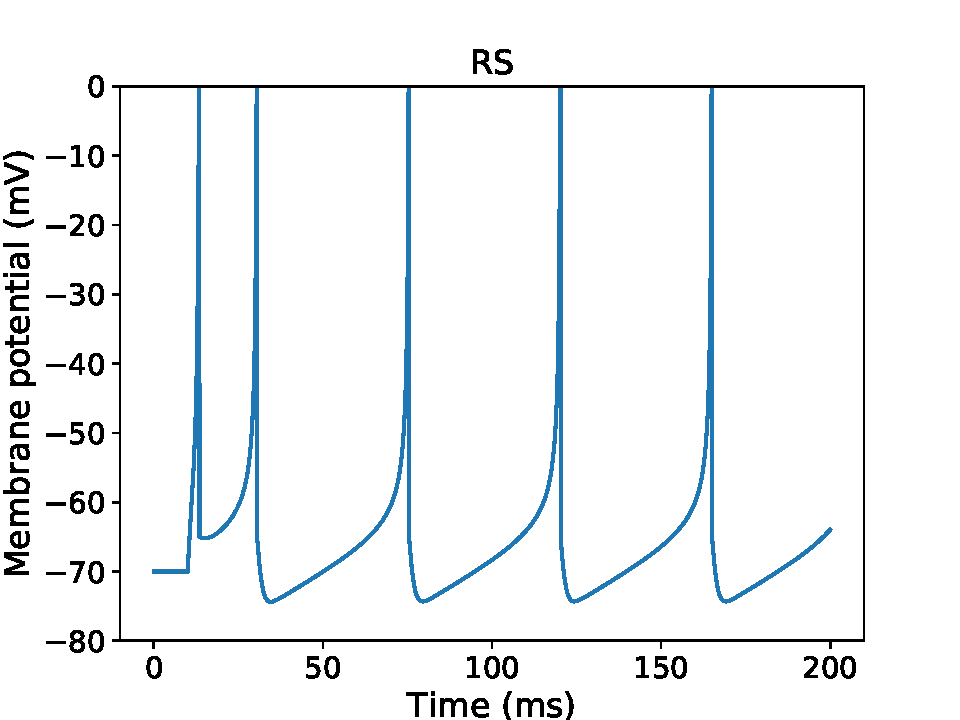
\includegraphics[scale = 0.4]{Iz_plots/RS}}
\caption{Replication of regular spiking behaviour.
The neuron is given an initial membrane potential of $-70mV$ and continuous DC source input, starting at $10ms$.}
\label{fig:RS}
\end{figure} 

The most common type of excitatory neuron in mammalians are regular spiking cells, that fire spikes with decreasing frequency. 
When given a regular, unchanging stimulus, such as a step current, the neuron will fire a few spikes with a short inter-spike period.
The inter-spike period will then increase over time, as the spiking frequency decreases. 

This is called spike-frequency adaptation. 
The frequency is relatively high at the onset and then it adapts.
It is caused by feedback (recurrent) inhibition within the network. 

\subsection{Fast Spiking}
\label{subsec:FS}
\begin{figure}[H]
\centering
\makebox[\textwidth]{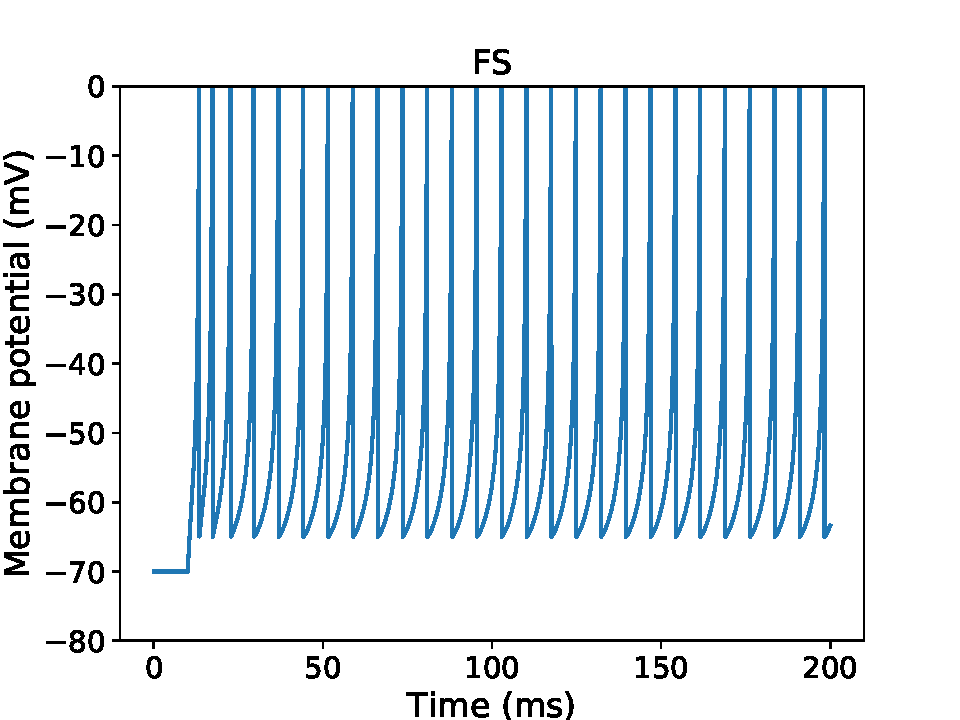
\includegraphics[scale = 0.4]{Iz_plots/FS}}
\caption{Replication of fast spiking behaviour.
The neuron is given an initial membrane potential of $-70mV$ and continuous DC source input, starting at $10ms$.}
\label{fig:FS}
\end{figure} 

The fast spiking behaviour is when a neuron fires with extremely high frequency without adaptation. 

\subsection{Low-threshold Spiking}
\label{subsec:LTS}
\begin{figure}[H]
\centering
\makebox[\textwidth]{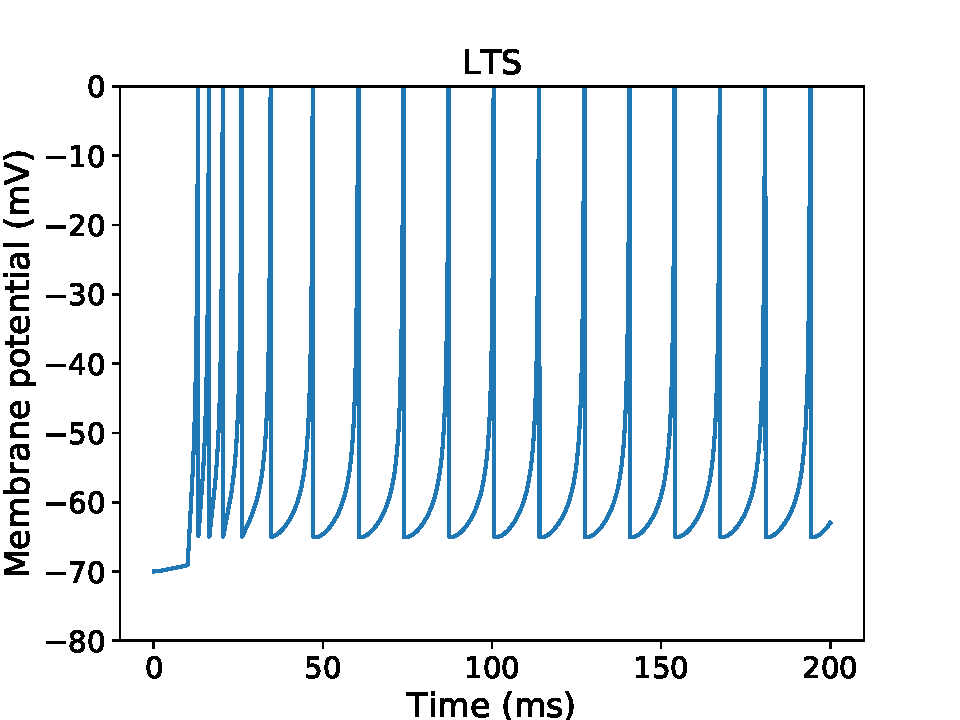
\includegraphics[scale = 0.4]{Iz_plots/LTS}}
\caption{Replication of low-threshold spiking behaviour.
The neuron is given an initial membrane potential of $-70mV$ and continuous DC source input, starting at $10ms$.}
\label{fig:LTS}
\end{figure} 

The low-threshold spiking behaviour is when a neuron fires with extremely high frequency with frequency adaptation (slowing down).

\subsection{Intrinsically Bursting}
\label{subsec:IB}
Bursting is a dynamic state where a neuron repeatedly fire in groups. 
It will fire a few spikes (more than two) and then have a period of quiescence (meaning a state where the neuron does not fire), before firing its next group of spikes. 

\begin{figure}[H]
\centering
\makebox[\textwidth]{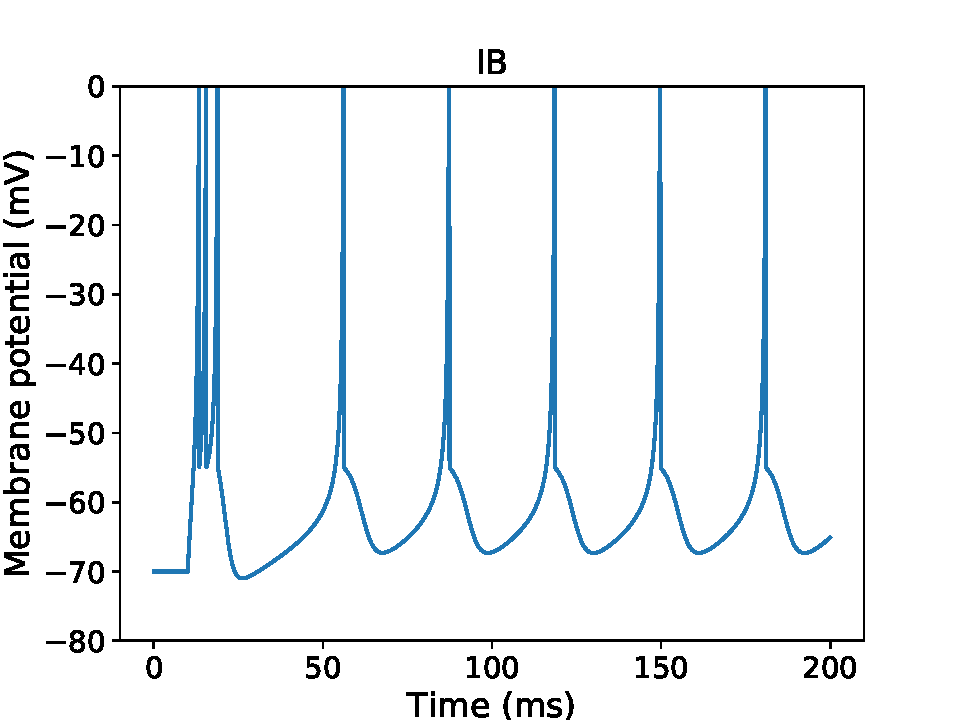
\includegraphics[scale = 0.4]{Iz_plots/IB}}
\caption{Replication of intrinsically bursting behaviour.
The neuron is given an initial membrane potential of $-70mV$ and continuous DC source input, starting at $10ms$.}
\label{fig:IB}
\end{figure} 
Intrinsically bursting is when a neuron fires an initial burst of spikes and then continues with shorter bursts. 
This behaviour then continues until the stimulus stops (tonic spiking)~\cite{Izhikevich:2006}.

\begin{figure}[H]
\centering
\makebox[\textwidth]{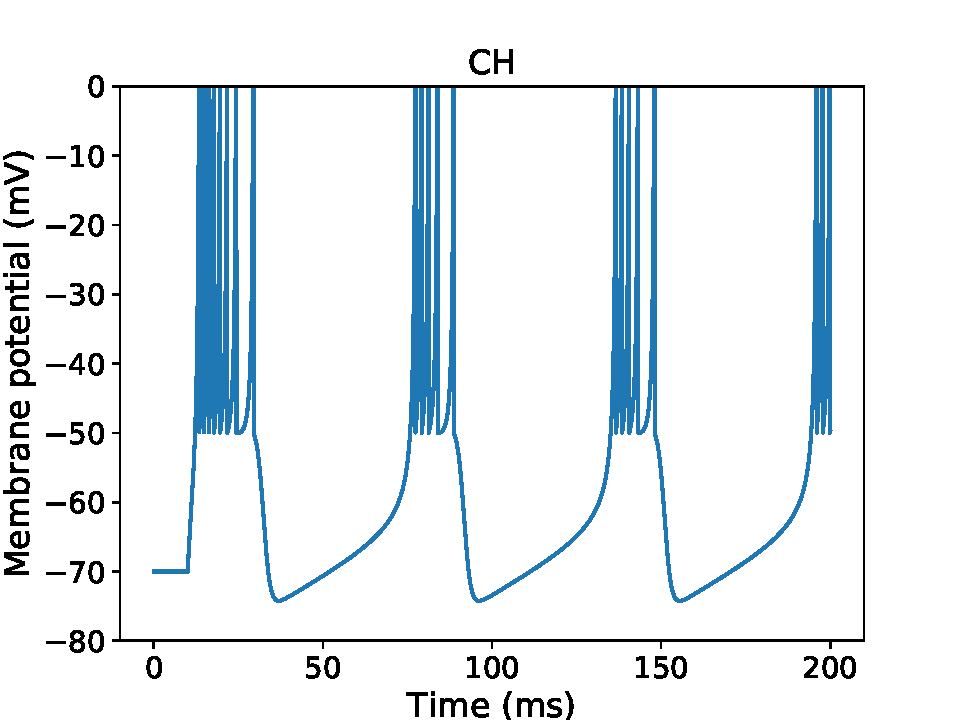
\includegraphics[scale = 0.4]{Iz_plots/CH}}
\caption{Replication of chattering behaviour.
The neuron is given an initial membrane potential of $-70mV$ and continuous DC source input, starting at $10ms$.}
\label{fig:CH}
\end{figure} 
Chattering neurons can fire high-frequency bursts with relatively short inter-burst periods. 

\begin{figure}[H]
\centering
\begin{minipage}{.45\textwidth}
\makebox[\textwidth]{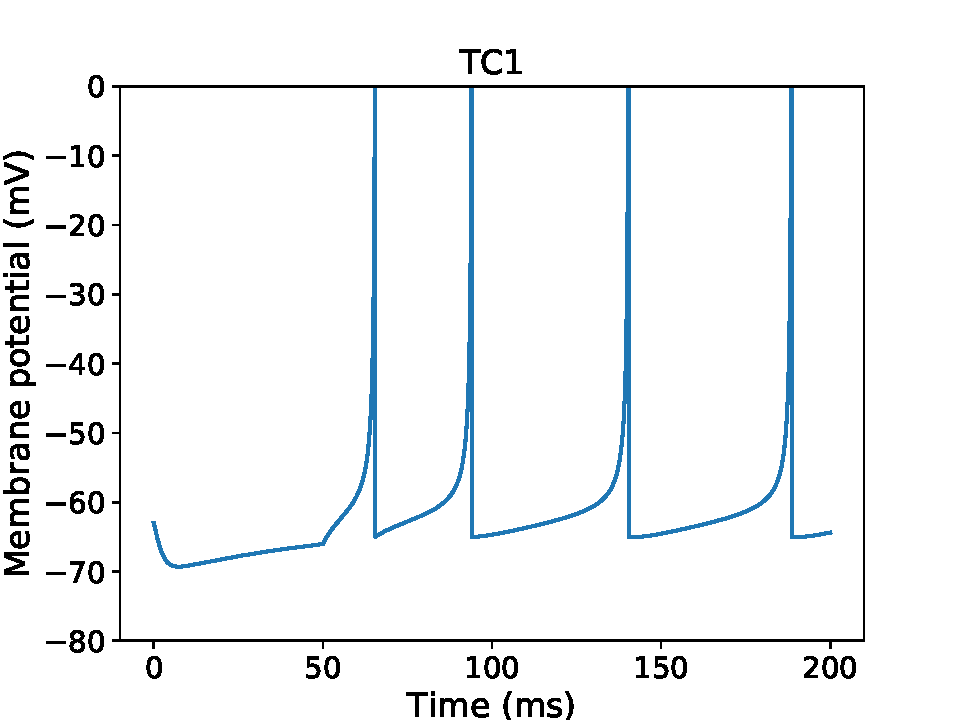
\includegraphics[scale = 0.4]{Iz_plots/TC1}}
\captionof{figure}{Initial membrane potential of $-63mV$ and continuous DC source input, starting at $50ms$.}
\label{fig:TC1}
\end{minipage}
\begin{minipage}{.45\textwidth}
\makebox[\textwidth]{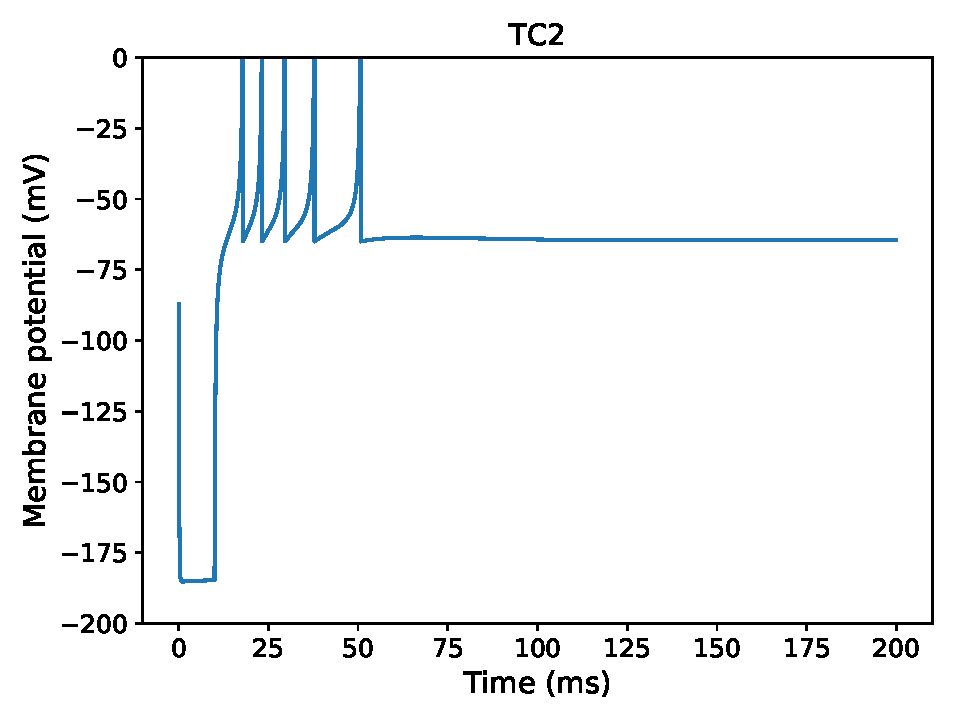
\includegraphics[scale = 0.4]{Iz_plots/TC2}}
\captionof{figure}{Initial membrane potential of $-87mV$ and negative step current input, starting at $10ms$.}
\label{fig:TC2}
\end{minipage}
\caption{Replication of Thalamo-Cortical neuron behaviours.}
\end{figure}
The Izhikevich model also reproduces the behaviour of Thalamo-cortical neurons.
Thalamo-cortical neurons will exhibit tonic spiking when they are at rest and then are depolarized by sufficient input, see figure~\ref{fig:TC1}. 
Although, if a negative input current is introduced the membrane potential will be hyperpolarized. 
The neurons react by firing a rebound burst of action potentials, see figure~\ref{fig:TC2}. 

\subsection{Resonance}
\label{subsec:RZ}
\begin{figure}[H]
\centering
\makebox[\textwidth]{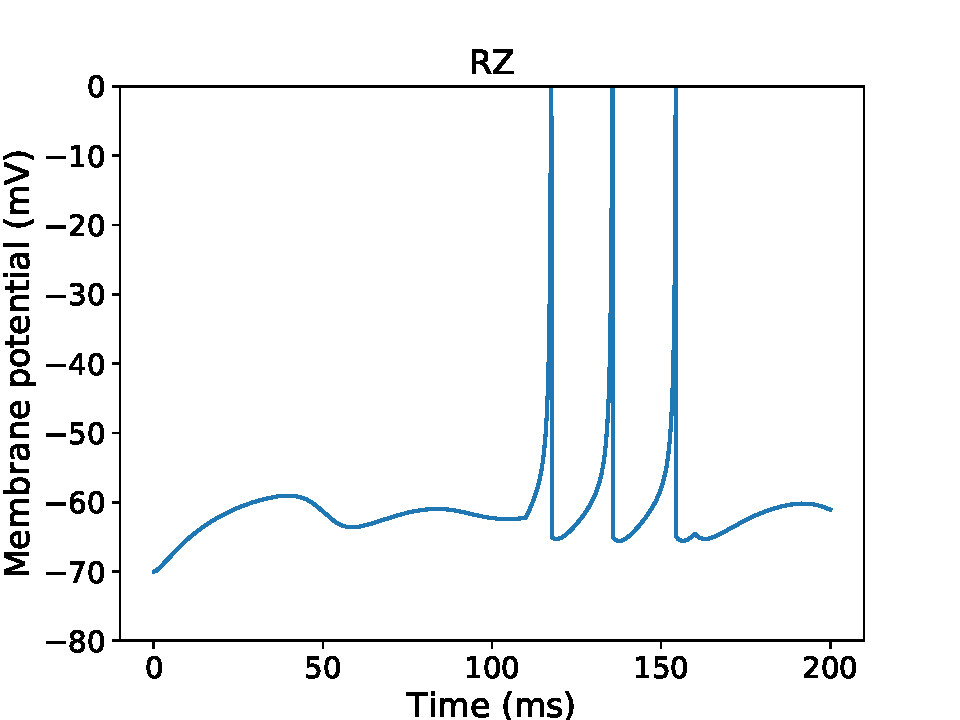
\includegraphics[scale = 0.4]{Iz_plots/RZ}}
\caption{Replication of resonator behaviour.
The neuron is given an initial membrane potential of $-70mV$ and DC source input, starting at $0.5ms$.
The input current increases at $110ms$ and then drops back down to its original amplitude.}
\label{fig:RZ}
\end{figure} 
Resonance behaviours in neurons indicates that they can discriminate between inputs.
The neurons respond selectively to inputs at the neurons preferred frequencies~\cite{hutcheon2000resonance}.
The replication in figure~\ref{fig:RZ} shows subthreshold oscillations.
The neuron then resonates to the appropriate input. 

\section{Izhikevich Mathematical Outline}
\label{sec:iterations}
Here I demonstrate how the model works by breaking down each step. 
The parameter values for the regular spiking neural behaviour (RS) were taken from the Izhikevich paper~\cite{izhikevich2003simple} and substituted into the equations \ref{eq:IZ1} and \ref{eq:IZ2}. 
The following outlines four iterations with the RS Izhikevich neuron, while applying the rules from equations \ref{eq:IZ3} and \ref{eq:IZ4}. \\

$1^{st}$ iteration ($p_1$):
\begin{align} \label{eq:1.5}
v'_{1} &= 0.04(\underbrace{-70}_{v_0})^2 + 5(\underbrace{-70}_{v_0}) + 140 - (\underbrace{-14}_{u_0}) + (\underbrace{25}_I) = 25 \nonumber \\
\nonumber \\
v_1 &= \underbrace{-70}_{v_0} + \underbrace{25}_{v'_{1}} = -45 mV \nonumber \\
\nonumber \\
u'_{1} &= \underbrace{0.02}_a\big((\underbrace{0.2}_b) \cdot (\underbrace{-70}_{v_0}) - (\underbrace{-14}_{u_0})\big) = 0 \nonumber \\
\nonumber \\
u_1 &= \underbrace{-14}_{u_0} + \underbrace{0}_{u'_{1}} = -14
\nonumber \\
\end{align}

$2^{nd}$ iteration ($p_2$):
\begin{align} \label{eq:1.6}
v'_{2} &= 0.04(\underbrace{-45}_{v_1})^2 + 5(\underbrace{-45}_{v_1}) + 140 - (\underbrace{-14}_{u_1}) + 25 = 35 \nonumber \\
\nonumber \\
v_2 &= \underbrace{-45}_{v_1} + \underbrace{35}_{v'_{2}} = -10 \nonumber \\
\nonumber \\
u'_{2} &= 0.02\big((0.2) \cdot (\underbrace{-45}_{v_1})-(\underbrace{-14}_{u_1})\big) = 0.1 \nonumber \\
\nonumber \\
u_2 &= \underbrace{-14}_{u_1} + \underbrace{0.1}_{u'_{2}} = -13.99  \nonumber \\
\end{align}

$3^{rd}$ iteration ($p_3$):
\begin{align} \label{eq:1.7}
v'_{3} &= 0.04(\underbrace{-10}_{v_2})^2 + 5(\underbrace{-10}_{v_2}) + 140 - (\underbrace{-13.99}_{u_2}) + 25 = 132.99 \nonumber \\
\nonumber \\
v_3 &= \underbrace{-10}_{v_2} + \underbrace{132.99}_{v'_3} = 122.99 \nonumber \\
\nonumber \\
u'_{3} &= 0.02\big((0.2) \cdot (\underbrace{-10}_{v_2})-(\underbrace{-13.99}_{u_2})\big) = 0.238 \nonumber \\
\nonumber \\
u_3 &= \underbrace{-13.99}_{u_2} + \underbrace{0.238}_{u'_3} = -13.752 \nonumber \\
\nonumber \\
v_3 \geq 30mV \nonumber \\
\nonumber \\
v_3 &= c = -65 mV \nonumber \\ 
\nonumber \\
u_3 &= \underbrace{-13.752}_{u_3} + \underbrace{8}_d = -5.662 \nonumber \\
\end{align}

$4^{th}$ iteration ($p_4$):
\begin{align} \label{eq:1.8}
v'_{4} &= 0.04(\underbrace{-65}_{v_3})^2 + 5(\underbrace{-65}_{v_3}) + 140 - (\underbrace{-5.662}_{u_3}) + 25 = 14.662 \nonumber \\
\nonumber \\
v_4 &= \underbrace{-65}_{v_3} + \underbrace{14.662}_{v'_4} = -50.338 \nonumber \\
\nonumber \\
u'_{4} &= 0.02\big((0.2) \cdot (\underbrace{-65}_{v_3})-(\underbrace{-5.662}_{u_3})\big) = -0.14676 \nonumber \\
\nonumber \\
u_4 &= \underbrace{-5.662}_{u_3} + \underbrace{-0.14676}_{u'_4} = -5.80876 
\nonumber \\
\end{align}

\begin{figure}[H]
\centering
\begin{tikzpicture}[scale=0.9]
\begin{axis}[
    axis lines = left,
    xlabel = {$v \: \: (mV)$},
    ylabel = {$dv/dt \: \: (mV/ms)$},
    ymin=-100
]
\addplot [
	restrict y to domain = {-100:300},
    domain=-100:30, 
    samples=100, 
    color=orange,
]
{0.04*(x^2) + 5*x + 140 - (-14) + 25};
\addlegendentry{$0.04v^2 + 5v + 140 - (-14) + 25$}

%points and labels for the four iterations
\addplot[red, mark=x, mark options={scale=1.5}] coordinates {(-70,25)} node[pin={[pin distance=0.5cm, pin edge={gray, dashed, -}, scale=0.8]270:{$p_1(-70,25)$}}]{};
\addplot[blue, mark=x, mark options={scale=1.5}] coordinates {(-45, 35)} node[pin={[pin distance=1.1cm, pin edge={gray, dashed, -}, scale=0.8]270:{$p_2(-45, 35)$}}]{};
\addplot[magenta, mark=x, mark options={scale=1.5}] coordinates {(-10, 132.99)} node[pin={[pin distance=1cm, pin edge={gray, dashed, -}, scale=0.8]270:{$p_3(-10, 132.99)$}}]{};
\addplot[cyan, mark=x, mark options={scale=1.5}] coordinates {(-65, 14.662)} node[pin={[pin distance=1.3cm, pin edge={gray, dashed, -}, scale=0.8]90:{$p_4(-65, 14.662)$}}]{};
\end{axis}
\end{tikzpicture} 
\caption{
The equation of the curve is equation \ref{eq:IZ1}, with the values $-14$ and $25$ substituted into $u$ and $I$ respectively.
Additionally, the points from the four iterations have been marked on the curve:
red:\eqref{eq:1.5}; blue:\eqref{eq:1.6}; magenta:\eqref{eq:1.7} and cyan:\eqref{eq:1.8}.
The coordinates are written as $p_n(v_{n-1}, v_{n})$.}
\label{fig:diffplot}
\end{figure}

As shown in the graph, $p_4$ is not on the curve.
This is one iteration after a spike has occurred, where the membrane potential reached the threshold and the values were reset, as per equations \eqref{eq:IZ3} and \eqref{eq:IZ4}.
I created a python script to determine the values for $v$ and $u$ and the total number of spikes ($s$) from any specified number of iterations ($p_n$). 
For example, $p_{125}(-65, -3.7919)$, $s = 9$.
The coordinates just after the first three spikes were determined using this script, see figure \ref{fig:curves}.

\begin{figure}[H]
\centering
\begin{tikzpicture}[scale=0.9]
\begin{axis}[
    axis lines = left,
    xlabel = {$v \: \: (mV)$},
    ylabel = {$dv/dt \: \: (mV/ms)$},
    ymin=-100,
    ymax=500
]
%original curve
\addplot [
	restrict y to domain = {-100:300},
    domain=-80:30, 
    samples=100, 
    color=orange,
]
{0.04*(x^2) + 5*x + 140 - (-14) + 25};
\addlegendentry{$0.04v^2 + 5v + 140 - (-14) + 25$}

%curve after first spike, p4
\addplot [
	restrict y to domain = {-100:300},
    domain=-80:30, 
    samples=100, 
    color=red,
]
{0.04*(x^2) + 5*x + 140 - (-5.662) + 25};
\addlegendentry{$0.04v^2 + 5v + 140 - (-5.662) + 25$}

%curve after second spike, p8
\addplot [
	restrict y to domain = {-100:300},
    domain=-80:30, 
    samples=100, 
    color=blue,
]
{0.04*(x^2) + 5*x + 140 - (2.332) + 25};
\addlegendentry{$0.04v^2 + 5v + 140 - (2.332) + 25$}

%curve after third spike, p13
\addplot [
	restrict y to domain = {-100:300},
    domain=-80:30, 
    samples=100, 
    color=magenta,
]
{0.04*(x^2) + 5*x + 140 - (9.268) + 25};
\addlegendentry{$0.04v^2 + 5v + 140 - (9.268) + 25$}

%coordinates of the points just after the first three spikes
\addplot[black, mark=x, mark options={scale=1.5}] coordinates {(-65, 14.662)};
\addplot[black, mark=x, mark options={scale=1.5}] coordinates {(-65, 6.6680422568)};
\addplot[black, mark=x, mark options={scale=1.5}] coordinates {(-65, -0.26841742317)};
\end{axis}
\end{tikzpicture} 
\caption{
The curves were created by updating the original equation (orange) for $v'$, using $p_4(-65, 14.662)$, $p_8(-65, 6.668)$ and $p_{13}(-65, -0.268)$.
}
\label{fig:curves}
\end{figure}

Figure \ref{fig:curves} shows that after every spike the curve shifts down, due to the dramatic change in the recovery variable $u$.

%Bibliography
\cleardoublepage
\phantomsection
\nocite{*}
\addcontentsline{toc}{chapter}{Bibliography}
\bibliographystyle{plain}
\bibliography{BibList}

\end{document}